% This is the Duke University Statistical Science LaTeX thesis template.
% It has been adapted from the Reed College LaTeX thesis template. The
% adaptation was done by Mine Cetinkaya-Rundel (MCR). Some of the comments
% that are specific to Reed College have been removed.
%
% Most of the work on the original Reed College document class and template
% was done by Sam Noble (SN). Later comments etc. by Ben Salzberg (BTS).
% Additional restructuring and APA support by Jess Youngberg (JY).
%
% See https://www.reed.edu/cis/help/latex/ for help. There are a
% great bunch of help pages there, with notes on
% getting started, bibtex, etc. Go there and read it if you're not
% already familiar with LaTeX.
%
% Any line that starts with a percent symbol is a comment.
% They won't show up in the document, and are useful for notes
% to yourself and explaining commands.
% Commenting also removes a line from the document;
% very handy for troubleshooting problems. -BTS

%%
%% Preamble
%%
% \documentclass{<something>} must begin each LaTeX document
\documentclass[12pt,twoside]{dukestatscithesis}
% Packages are extensions to the basic LaTeX functions. Whatever you
% want to typeset, there is probably a package out there for it.
% Chemistry (chemtex), screenplays, you name it.
% Check out CTAN to see: http://www.ctan.org/
%%
\usepackage{graphicx,latexsym}
\usepackage{amsmath}
\usepackage{amssymb,amsthm}
\usepackage{longtable,booktabs,setspace}
\usepackage{chemarr} %% Useful for one reaction arrow, useless if you're not a chem major
\usepackage[hyphens]{url}
% Added by CII
\usepackage{hyperref}
\usepackage{lmodern}
\usepackage{float}
\floatplacement{figure}{H}
% End of CII addition
\usepackage{rotating}

% Next line commented out by CII
%%% \usepackage{natbib}
% Comment out the natbib line above and uncomment the following two lines to use the new
% biblatex-chicago style, for Chicago A. Also make some changes at the end where the
% bibliography is included.
%\usepackage{biblatex-chicago}
%\bibliography{thesis}


% Added by CII (Thanks, Hadley!)
% Use ref for internal links
\renewcommand{\hyperref}[2][???]{\autoref{#1}}
\def\chapterautorefname{Chapter}
\def\sectionautorefname{Section}
\def\subsectionautorefname{Subsection}
% End of CII addition

% Added by CII
\usepackage{caption}
\captionsetup{width=5in}
% End of CII addition

% \usepackage{times} % other fonts are available like times, bookman, charter, palatino


% To pass between YAML and LaTeX the dollar signs are added by CII
\title{Examining Injustice in Environmental Toxicity}
\author{Anne Driscoll}
% The month and year that you submit your FINAL draft TO THE LIBRARY (May or December)
\date{May 2018}
\advisor{David Banks}
\institution{Duke University}
\degree{Bachelor of Science in Statistical Science}
\committeememberone{Committeemember O. Name}
\committeemembertwo{Committeemember T. Name}
\dus{Mine Cetinkaya Rundel}
%If you have two advisors for some reason, you can use the following
% Uncommented out by CII
% End of CII addition

%%% Remember to use the correct department!
\department{Department of Statistical Science}

% Added by CII
%%% Copied from knitr
%% maxwidth is the original width if it's less than linewidth
%% otherwise use linewidth (to make sure the graphics do not exceed the margin)
\makeatletter
\def\maxwidth{ %
  \ifdim\Gin@nat@width>\linewidth
    \linewidth
  \else
    \Gin@nat@width
  \fi
}
\makeatother

\renewcommand{\contentsname}{Table of Contents}
% End of CII addition

\setlength{\parskip}{0pt}

% Added by CII
  %\setlength{\parskip}{\baselineskip}
  \usepackage[parfill]{parskip}

\providecommand{\tightlist}{%
  \setlength{\itemsep}{0pt}\setlength{\parskip}{0pt}}

\Acknowledgements{
I want to thank a few people.
}

\Dedication{
You can have a dedication here if you wish.
}

\Preface{
This is an example of a thesis setup to use the reed thesis document
class (for LaTeX) and the R bookdown package, in general.
}

\Abstract{
The preface pretty much says it all. \par

Second paragraph of abstract starts here.
}

% End of CII addition
%%
%% End Preamble
%%
%

\usepackage{amsthm}
\newtheorem{theorem}{Theorem}[chapter]
\newtheorem{lemma}{Lemma}[chapter]
\theoremstyle{definition}
\newtheorem{definition}{Definition}[chapter]
\newtheorem{corollary}{Corollary}[chapter]
\newtheorem{proposition}{Proposition}[chapter]
\theoremstyle{definition}
\newtheorem{example}{Example}[chapter]
\theoremstyle{definition}
\newtheorem{exercise}{Exercise}[chapter]
\theoremstyle{remark}
\newtheorem*{remark}{Remark}
\newtheorem*{solution}{Solution}
\begin{document}

% Everything below added by CII
  \maketitle

\frontmatter % this stuff will be roman-numbered
\pagestyle{empty} % this removes page numbers from the frontmatter
  \begin{acknowledgements}
    I want to thank a few people.
  \end{acknowledgements}
  \begin{preface}
    This is an example of a thesis setup to use the reed thesis document
    class (for LaTeX) and the R bookdown package, in general.
  \end{preface}
  \hypersetup{linkcolor=black}
  \setcounter{tocdepth}{2}
  \tableofcontents

  \listoftables

  \listoffigures
  \begin{abstract}
    The preface pretty much says it all. \par
    
    Second paragraph of abstract starts here.
  \end{abstract}
  \begin{dedication}
    You can have a dedication here if you wish.
  \end{dedication}
\mainmatter % here the regular arabic numbering starts
\pagestyle{fancyplain} % turns page numbering back on

\chapter*{Introduction}\label{introduction}
\addcontentsline{toc}{chapter}{Introduction}

Environmental justice literature has focused largely on the motivations
and policy approaches to help account for the disproportionate burden of
environmental hazards on minority communities. The questions being asked
are critical to building a knowledge base that allows us to create
policy that helps correct the problem of hazard allocation, but aren't
significantly addressing the canges in the hazard burden over time as it
relates to policy already in place and natural sorting.

This thesis seeks to address the investigative question of if minority
communities have experienced substantial reductions in their relative
environmental toxicity, when those shifts are occuring, and a look in to
the traits that are predictive of high environmental toxicity.

\section{Keywords}\label{keywords}

Environmental Inequality, Racial Inequality, Non-parametric analysis

\chapter{Introduction to Environmental Justice}\label{rmd-basics}

testing testing

123

\chapter{Data}\label{math}

\section{Raw Data}\label{raw-data}

The Risk Screening Environmental Indicators (RSEI) Model is a very
detailed data set produced by the Environmental Protection Agency (EPA).
It is based upon the Toxic Release Inventory (TRI), which (for about 30
years) has been. The TRI program manages the regulations, policies and
facilities that are ultimately reported.

TRI data is self reported, with each observation being a release of a
reporting facility for a reporting chemical. For each observation, data
is collected on which chemical was released, how much of it was
released, and the specific facility from which it was released.

The detailed location and chemical data that is collected through TRI,
as well as detailed weather data from NOAA is reformatted through a fate
and transport model across an 800m grid across the USA to create the
RSEI data. The ultimate data we have access to through the RSEI data is
an observation for each release, for each square in the grid the release
hits. This gives us an idea of how the chemicals spread from the release
locations, and enables us to create a map across the entire nation for
where TRI chemicals are spreading at any time between 1988 and 2014.

\section{Important Caveats}\label{important-caveats}

Due to the nature of the data, there are a few interesting caveats to
consider.
\begin{itemize}
\item
  The RSEI data is self reported, and has been thought to contain some
  severe underreporting.
\item
  The data is entirely based off a black box fate and transport model.
  The model has uncertainty that we are not addressing.
\item
  The data only captures releases from certain industries, for certain
  facility types within those industries, for certain chemical types
  within those facilities. Not all chemicals are mandated reporting, and
  any analysis that is done based off the data can't be extrapolated to
  discuss toxicity more generally.
\item
  Not only does the data not capture all chemicals, it also doesn't
  broach many common nuicances, both enviromental and toxic. Because of
  this, it is difficult to relate the RSEI scores to health outcomes in
  an area. In discussion of hte toxicity, it is worth noting that
  certain toxicity types may not present themselves as easily (eg. may
  or may not reach local water systems). There are also more obvious
  environmental hazards, that are likely to have strong influence on
  public health and living conditions that TRI doesn't address, eg:
  brownfields, solid waste disposal, animal farming, hazardous waste,
  etc.
\item
  RSEI gives the weight of the release and the chemical of the release,
  but as chemicals have very different levels of toxicity. To that end,
  the EPA assigned each chemical a `toxicity' weight, by which the
  amount of the chemical is multiplied. This means that we can aggregate
  all the chemicals in an area, and compare the overall toxicity over
  space and time. The toxicity weights allow us to compare locations,
  but also means that the values only have meaning in comparison.
\end{itemize}
Despite the limitations that the data presents, it provides an
incredibly detailed and complex view of toxicity in America that is
worth delving in to.

\section{Consistency in Reporting (detailed data
description)}\label{consistency-in-reporting-detailed-data-description}

\subsection{Census Comparability}\label{census-comparability}

For the time period that RSEI data is available during (1988 - 2014),
Census geographies have experienced considerable overhaul. Many of our
questions of interest involve demographics, and the changes we see in
environmental toxicity over time for those demographics. As such, we
need to be able to aggregate the toxicity to block group or tract level
to be able to merge with Census data. As such, we caluclate the toxicity
values for each geographic unit for the closest temporal census
geography (1990, 2000 or 2010).

\subsection{Details of Chemical
Consistency}\label{details-of-chemical-consistency}

Using the consistent\_chemicals table provided by Rich Puchalsky, the
chemicals that are relevant to the specific years of interest are
calculated in the runDatabase.R file in the
define\_consistent\_chemicals function. They are found by selecting the
subset of chemicals where the year of initial regulation is before the
interest period, and the year of deregulation is after the interest
period, while also excluding delisted chemicals.

\subsection{Details of NAICS Code
Consistency}\label{details-of-naics-code-consistency}

NAICS codes are a form of industry code. In the RSEI data the only NAICS
code reference is in the facility data table. This table provides a list
of 6 NAICS codes that are most relevant to the facility. However, NAICS
codes are release specific, not facility specific, meaning that for each
emission reported a NAICS code is reported. Since NAICS codes are
regulated independently of chemical codes, NAICS codes that are not
consistently reported across the time period of interest must be removed
to maintain continuity. For a toy example, a textiles facility releasing
mercury might have to report it, but the neighboring mining facility
might not. If that changes over the time period, and suddenly mining
needs to report, we will see an artificial huge jump in the mercury
present in that area if we don't remove by industry. Removing by
facility is also not accurate, since facilities might have different
types of NAICS emissions. The textiles facility might make both shoes
and jackets, with different industry codes and therefore different
reporting requirements.

To get data on the NAICS codes by submission, data must be taken from
the original TRI data, and linked to the microdata by the submission and
release tables. The Document Control Number (doc\_ctrl\_num) and
Industry Code (industry\_code) columns from the Submission NAICS Codes
(v\_tri\_submission\_naics) table provide the information necessary to
link to our microdata.

\section{Ultimate Data Form}\label{ultimate-data-form}

The initial data from RSEI is in the form of one observation per release
per block on the 800m grid that it hit. Given that the 800m grid across
the United States has on the order of 10 billion squares, each release
hits many squares, we have many releases, and the data covers 27 years,
this is an enormous data set. Overall, the disaggregated microdata is
approximately 4 terabytes of data.

In the data cleansing process, we filter the data to remove industries
and chemicals that were not consistent over the period of inquiry, and
aggregate the data to the relevant Census geographies. The data, after
an extensive and computationally intesive process, forms a data set with
an observation for each year, for each block group/tract, with just a
toxicity level.

The pollution estimate must be interpreted in the context of the
consistency adjustments. For example, towns with extremely high mining
emissions may not show as exceptionally high pollution, as mining is one
of the industries that had different regulations over the 1990-2010 time
period, and therefore the reported mining emissions have been removed
entirely. Essentially, the pollution estimates are comparable across
time and location, but only in the context of continuous EPA regulation.

\chapter{Approaches and Methods}\label{ref-labels}

\section{Geographic Level of
Analysis}\label{geographic-level-of-analysis}

The questions we would like to pose - how the distributions of toxicity
that individuals experience over time are predicted by their complex,
multidimensional identities - is inherently intended to be a person
level analysis. That intent may not be achievable given the available
data.

This analysis depends on two data sources, the disaggregated RSEI toxic
release data as compiled to contain only releases that are consistently
reported between 1990 and 2010, as well as relevant demographic
information from the census.

RSEI environmental data can be obtained at extremely fine level (the 800
meter grid across the United States,) but the finest grain Census data
is available at is the block level, which contains between 0 and a few
hundred people. At such low geographic levels, few variables are
available for demographics due to identifiability concerns.
Additionally, few cross tabulations are available, due to concerns of
identifiability. Using a low level of geography (like census blocks or
block groups) is important for the environmental aspect of this
analysis, since environmental hazards can be very localized, especially
along neighborhood lines in urban areas.

Unfortunately, the availability of cross tabulations is equally
important to the goal of this work in examining inequality of
environmental burden held by minority groups in America. The
intersection of social identies, especially those steeped in systems of
oppression, is extremely important for identifying unequal burdens. For
example, low income populations across the board may be more likely to
experience environmental hazards, but low income minority populations
could be much more likely than low income white populations to
experience extreme hazard. The intersections of demographic
charictersitics, such as race and income or race and education are
likely to be important in teasing out differences true inequality
burden.

To combine the data, we assign the aggregated releases to their
respective geographies. For each census geography, we also have
estimates of number of various population groups. From there, we move to
a person level analysis by assigning each of the people the toxicity for
the geography they originated in. By assigning each person the toxicity
of their block group, we can aggregate nationally to find the
distribution of toxicity that each group experiences. This approach is
restricted in ability to approach the problem in an intersectional
manner, since we can only build a distribution for each of the crosstabs
we have available. For higher levels of geography (where we might, for
example, have race by income) we would be able to build national
distributions for each income by race group.

In choosing the level of aggregation at which to assign toxicity, in
order to balance the needs of accuracy of toxicity and availability of
cross tabulations, we create the overall toxicity distribution for
Americans by assigning each individual a toxicity level for each level
of geography. Using block group as the smallest form of geography, and
aggregating up to state (including tract and county in between) we see
how the distribution changes at each level of aggregation.

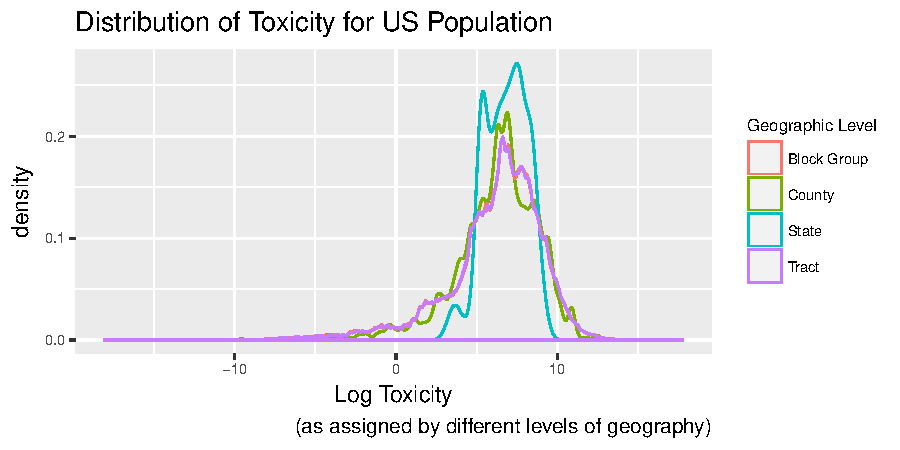
\includegraphics{thesis_files/figure-latex/unnamed-chunk-2-1.pdf}

We see expected results when looking at the aggregation at state level.
Given that we are assigning each individual the mean toxicity in their
entire state, we are eliminating most of the variation from the data.
States seem to have overall similar toxicity levels, but interestingly
the tract data seems to build a distribution very similar to the block
group level assignment. This may be because the block group level is
aggregating a large group of our fine grain toxicity data, and has
therefore already lost the street block by street block variation that
we had deemed so crucial, so aggregating several block groups leaves us
in a similar neighborhood level of aggregation.

\section{Temporal Level of Analysis}\label{temporal-level-of-analysis}

\section{Non-Parametric Analysis}\label{non-parametric-analysis}

\section{Trends Over Time}\label{trends-over-time}
\begin{Shaded}
\begin{Highlighting}[]
\NormalTok{vars =}\StringTok{ }\KeywordTok{c}\NormalTok{(}\StringTok{"white"}\NormalTok{, }\StringTok{"black"}\NormalTok{, }\StringTok{"hispanic"}\NormalTok{, }\StringTok{"owners"}\NormalTok{, }\StringTok{"renters"}\NormalTok{)}
\NormalTok{p1990 =}\StringTok{ }\NormalTok{t1990}
\NormalTok{p1990[vars] =}\StringTok{ }\NormalTok{p1990[vars]/p1990$tot_pop}
\NormalTok{p1990$density =}\StringTok{ }\NormalTok{p1990$tot_pop/p1990$area}
\NormalTok{m =}\StringTok{ }\KeywordTok{lm}\NormalTok{(lconcentration ~}\StringTok{ }\DecValTok{1} \NormalTok{+}\StringTok{ }\NormalTok{owners +}\StringTok{ }\NormalTok{renters +}\StringTok{ }\NormalTok{black +}\StringTok{ }\NormalTok{hispanic +}\StringTok{ }\NormalTok{density, }\DataTypeTok{data =} \NormalTok{p1990)}

\NormalTok{p2010 =}\StringTok{ }\NormalTok{t2010}
\NormalTok{p2010[vars] =}\StringTok{ }\NormalTok{p2010[vars]/p2010$tot_pop}
\NormalTok{p2010$density =}\StringTok{ }\NormalTok{p2010$tot_pop/p2010$area}
\NormalTok{m =}\StringTok{ }\KeywordTok{lm}\NormalTok{(lconcentration ~}\StringTok{ }\DecValTok{1} \NormalTok{+}\StringTok{ }\NormalTok{owners +}\StringTok{ }\NormalTok{renters +}\StringTok{ }\NormalTok{black +}\StringTok{ }\NormalTok{hispanic +}\StringTok{ }\NormalTok{density, }\DataTypeTok{data =} \NormalTok{p2010)}
\end{Highlighting}
\end{Shaded}
\chapter{Results}\label{organization}

testing testing

123

\chapter*{Conclusion}\label{conclusion}
\addcontentsline{toc}{chapter}{Conclusion}

testing testing

123 hello

\appendix

\chapter{Code Appendix}\label{code-appendix}

This appendix includes all of the R chunks of code that were hidden
throughout the document (using the \texttt{include\ =\ FALSE} chunk tag)
to help with readibility and/or setup.

\textbf{In the main Rmd file}
\begin{Shaded}
\begin{Highlighting}[]
\CommentTok{# This chunk ensures that the thesisdowndss package is}
\CommentTok{# installed and loaded. This thesisdowndss package includes}
\CommentTok{# the template files for the thesis.}
\NormalTok{if(!}\KeywordTok{require}\NormalTok{(devtools))}
  \KeywordTok{install.packages}\NormalTok{(}\StringTok{"devtools"}\NormalTok{, }\DataTypeTok{repos =} \StringTok{"http://cran.rstudio.com"}\NormalTok{)}
\NormalTok{if(!}\KeywordTok{require}\NormalTok{(thesisdowndss))}
  \NormalTok{devtools::}\KeywordTok{install_github}\NormalTok{(}\StringTok{"mine-cetinkaya-rundel/thesisdowndss"}\NormalTok{)}
\KeywordTok{library}\NormalTok{(thesisdowndss)}
\end{Highlighting}
\end{Shaded}
\textbf{In Chapter \ref{ref-labels}:}

\backmatter

\chapter*{References}\label{references}
\addcontentsline{toc}{chapter}{References}

\markboth{References}{References}

\noindent

\setlength{\parindent}{-0.20in} \setlength{\leftskip}{0.20in}
\setlength{\parskip}{8pt}

\hypertarget{refs}{}
\hypertarget{ref-angel2000}{}
Angel, E. (2000). \emph{Interactive computer graphics : A top-down
approach with opengl}. Boston, MA: Addison Wesley Longman.

\hypertarget{ref-angel2001}{}
Angel, E. (2001a). \emph{Batch-file computer graphics : A bottom-up
approach with quicktime}. Boston, MA: Wesley Addison Longman.

\hypertarget{ref-angel2002a}{}
Angel, E. (2001b). \emph{Test second book by angel}. Boston, MA: Wesley
Addison Longman.


% Index?

\end{document}
